\documentclass[12pt]{article}
\usepackage{graphicx}
\usepackage{titletoc}
\usepackage{fancyhdr}
\usepackage{tocloft}
\usepackage[a4paper, inner=1.5in, outer=1.25in, top=1.5in, bottom=1in, left=1.5in, right=1in]{geometry}
\usepackage[onehalfspacing]{setspace}

\usepackage{biblatex}
\addbibresource{Proposal/references.bib}
\defbibheading{mybibliography}[\refname]{%
  \section*{\centering\MakeUppercase{\Large\bfseries #1}}%
  \addcontentsline{toc}{section}{\MakeUppercase{#1}}}

% Custom formatting for the table of contents title
\renewcommand{\contentsname}{\centering\textbf{CONTENTS}}

\begin{document}

\begin{center} 
        {\fontsize{14pt}{20}\selectfont \textbf{\MakeUppercase{Tribhuvan University}}}\\
        {\fontsize{14pt}{20}\selectfont \textbf{\MakeUppercase{institute of engineering}}}
        \vspace{0.4in}
\end{center}
\begin{figure}[h]
\centering
    
\includegraphics[width = 2.5in]{Proposal/static/LECLogo.jpg}
    \vspace{0.4in}
    \begin{center}
        \vspace{2mm}
        {\fontsize{14pt}{20}\selectfont \textbf{\MakeUppercase{Lalitpur Engineering College}}}
        \vspace{2mm}
        
        {\fontsize{14pt}{5}\selectfont \textbf{\MakeUppercase{Chakupat, lalitpur}}}
    \end{center}
    \vspace{0.4in}
\begin{center}
{\fontsize{14pt}{20}\selectfont \textbf{\MakeUppercase{a proposal on the project titled}}}\\
{\fontsize{14pt}{20}\selectfont \textbf{SAP: System Administration Portal}}\\
\vspace{0.6in}
    {\fontsize{14pt}{20}\selectfont \textbf{\MakeUppercase{submitted by:}}}\\
    {\fontsize{14pt}{20}\selectfont \textbf{Prabin Joshi [LEC077BCT012]}}\\
\vspace{0.6in}
    {\fontsize{14pt}{20}\selectfont \textbf{\MakeUppercase{submitted to:}}}\\
    {\fontsize{14pt}{20}\selectfont \textbf{Department of Computer Engineering}}\\
\vspace{0.6in}
    {\fontsize{14pt}{20}\selectfont \textbf{2023}}\\
\end{center}
\end{figure}
\thispagestyle{empty}
\newpage

\begin{center}
{\fontsize{12pt}{20}\selectfont A Proposal on the Project Titled}\\
\vspace{1in}
{\fontsize{14pt}{20}\selectfont \textbf{SAP: System Administration Portal}}\\
\vspace{1in}
Submitted as a part of requirement of \\the curriculum of
Software Engineering\\
\vspace{1in}
    {\fontsize{14pt}{20}\selectfont \textbf{\MakeUppercase{submitted by:}}}\\
    {\fontsize{14pt}{20}\selectfont \textbf{Prabin Joshi [LEC077BCT012]}}\\
\vspace{1in}
    {\fontsize{14pt}{20}\selectfont \textbf{\MakeUppercase{under the supervision of:}}}\\
    {\fontsize{14pt}{20}\selectfont \textbf{Bisikha Subedi}}\\
\vspace{1in}
{\fontsize{14pt}{20}\selectfont \textbf{13th August,2023}}\\
\end{center}
\thispagestyle{empty}
\newpage

\pagenumbering{Roman}
\begin{center}
\section*{\textbf{ABSTRACT}}
\end{center}
In the dynamic landscape of modern technology, efficient system administration is paramount for maintaining the stability, security and simplicity of any infrastructure. This proposal introduces a comprehensive System Administration Portal (SAP) designed to change the way organizations manage their resources, streamline administrative tasks, and enhance overall productivity. The System Administration Portal (SAP) is a central hub designed to simplify the complexities of technology management on campus. It offers a user-friendly interface that enables students to take control of various aspects of their tech ecosystem, all through an easy-to-navigate dashboard. By consolidating essential functions, the SAP eliminates the frustration of dealing with scattered tools and resources, making tech management accessible to students with varying levels of technical expertise.
The proposed Student System Administration Portal (SAP) aims to empower students with the tools they need to succeed in their academic endeavors. By simplifying tech management, fostering collaboration, and promoting a secure digital environment, the SAP contributes to a more productive and engaging college experience. Educational institutions stand to benefit from increased student satisfaction, enhanced tech literacy, and streamlined IT operations, reduced human efforts, making this proposal a compelling investment in the future of student-centered technology management.\\ \\
\textbf{Keywords}: \textit{SAP}, \textit{Dashboard}
\addcontentsline{toc}{section}{\textbf{ABSTRACT}}

\newpage

\addcontentsline{toc}{section}{\textbf{CONTENTS}}
\tableofcontents
\newpage

\renewcommand{\cftloftitlefont}{\hfill\Large\bfseries\MakeUppercase}
\renewcommand{\cftafterloftitle}{\hfill}
\listoffigures
\addcontentsline{toc}{section}{\textbf{LIST OF FIGURES}}
\newpage
\begin{center}
\section*{ABBREVIATIONS}
\begin{table}[h]
    \begin{tabular}{l l}
         SAP & \hspace{2in} System Administration Portal \vspace{2mm} \\
         MERN & \hspace{2in} MongoDB, Express JS, React JS, Node JS \vspace{2mm} \\
    \end{tabular}
\end{table}
\end{center}
\addcontentsline{toc}{section}{\textbf{ABBREVIATIONS}}
\newpage


\pagenumbering{arabic}

\begin{center}
\section{INTRODUCTION}
\end{center}
\subsection{Background}
The resources for students to study is something that is scattered throughout the Internet, in the form of Youtube videos, Drive links and so on. It is not practical to expect them to know exactly what they'll need and when they'll need it. It's common for students to start panicking while looking for those resources when actual work is to be done. It is a time consuming process and not very amiable to deadlines. It makes students' stressed and unable to focus on the task ahead, hampering their efficiency severely.
The proposed web application provides students with a centralized portal to access resources, collaborate within virtual rooms, and streamline their activities. This will mitigate the aforementioned problem. By creating a user-friendly and feature-rich platform, we can enhance the educational journey by improving outcomes, and helping students to thrive in their academic pursuits.
\newpage

\subsection{Problem Statement}
The proposed development of the System Administration Portal (SAP) addresses multiple pressing challenges within the current student academic landscape. Our students face a fragmented environment where essential course resources, assignments, and collaboration tools are scattered across various platforms, causing navigation complexities and inefficiencies. The absence of a unified resource management system results in disorganized materials, leading to confusion and difficulties in locating crucial information. This, coupled with a lack of interactive features, hampers student engagement and motivation, ultimately impacting retention rates. Instructors also encounter inefficiencies in updating resources, assessing student engagement, and providing timely feedback. Moreover, the current systems' limited support for distance learning leaves students and instructors ill-equipped to adapt to remote or hybrid educational models. Furthermore, technology literacy needs remain largely unmet, hindering students' preparation for the digital workforce. Privacy, security concerns, and inconsistent access control also arise due to the absence of a centralized platform, further exacerbating the challenges.
\newpage

\subsection{Scope}
The scope of SAP encompasses a wide array of features and functionalities designed to revolutionize the student academic experience. At its core, SAP will serve as a centralized online platform, providing students with streamlined access to a diverse range of resources, including course materials, assignments, research materials, and interactive tools, all within organized virtual rooms. This scope extends to fostering collaboration among students, instructors, and project teams, facilitating real-time interactions, discussions, and knowledge sharing. The portal will also feature personalized dashboards, empowering students to customize their learning journey by choosing relevant rooms aligned with their academic goals. Notifications and updates will be integrated into the platform, ensuring timely communication regarding deadlines, announcements, and resource changes. Additionally, the SAP will support distance learning initiatives, bridging the gap between physical and virtual classrooms. The application's capabilities extend to empowering instructors as well, offering real-time resource updates, engagement monitoring, and data-driven insights for improved teaching strategies. In a broader context, the SAP aims to enhance technology literacy, optimize resource management, promote student engagement, and foster a thriving educational ecosystem.
\newpage

\subsection{Objective}
\begin{itemize}
    \item To provide a user-friendly platform where students can access resources, collaborate within virtual rooms, and receive timely updates.
    \item To streamline resource management and enhance administrative efficiency.
\end{itemize}
\newpage

\begin{center}
\section{LITERARY REVIEW}
\end{center}
In the field of academia, efficiency is one of the core mantra. To make learning more and more efficient, we have witnessed a surge in the development of online platforms to facilitate just that. In this very field, we aim to provide a simple, smart and secure solution.
\vspace{0.2in}

\subsection{Existing}
\textbf{Canvas by Instructure:}\\
 "Canvas" by Instructure is a widely adopted Learning Management System (LMS) used by educational institutions globally. Canvas streamlines resource distribution, course management, and student interaction, much like the SAP's objectives. Canvas has demonstrated the value of providing students and educators with a unified space to access course materials, interact with peers, submit assignments, and receive feedback, all contributing to enhanced student engagement and academic outcomes.\cite{canvas}\\
 \\
 \textbf{Microsoft Teams:}\\
 Microsoft Teams, which, while originally designed for team collaboration in professional settings, has gained traction in the educational sector. With features like virtual rooms, document sharing, and real-time communication, Teams mirrors the collaborative aspects of the SAP proposal. The platform's versatility showcases the effectiveness of a comprehensive tool in fostering interaction and resource sharing among users, aligning with the SAP's vision of fostering student collaboration.\cite{microsoft}
 \newpage

 \subsection{Proposed}
 The proposed SAP aims to build upon the strengths of existing platforms while addressing specific challenges unique to the student academic experience. By integrating resource management, virtual room collaboration, personalized dashboards, and timely notifications, the SAP offers a holistic approach to student engagement and academic success. This is a step towards bridging the gap between classroom and remote learning, promoting technology literacy, and empowering both students and instructors to optimize their educational journey.\\
 The integration of resource management within the SAP ensures that students have a consolidated platform to access course materials, assignments, and reference materials, eliminating the frustration of navigating multiple systems. The inclusion of virtual room collaboration goes beyond mere content distribution, creating interactive spaces where students can discuss topics, collaborate on projects, and learn from one another, fostering a sense of community and active participation.

 \subsubsection{Functional Requirements:}
    \begin{itemize}
        \item The system must allow students, instructors, and administrators to log in securely with their unique credentials.
        \item The system should support password reset functionality.
        \item Students and instructors should be able to join rooms based on their courses or interests.
        \item Instructors must have the ability to create, modify, and manage rooms.
        \item Each room should display relevant information, such as room name, capacity, and resources available.
        \item Students in a room should be able to access resources such as files, links, and educational materials relevant to that room.
        \item Instructors should be able to upload and manage resources for their respective rooms.
        \item Administrators should be notified of access requests and have the ability to approve or deny them.
        \item The system should send timely notifications to users about room updates, resource availability, and access request status.
    \end{itemize}

    \subsubsection{Non-functional Requirements:}
    \begin{itemize}
        \item User data (including login credentials) must be securely stored and transmitted.
        \item Access to resources should be restricted based on room membership or authorization.
        \item The system should be responsive and capable of handling a large number of concurrent users without significant performance degradation.
        \item The user interface should be intuitive, easy to navigate, and visually appealing.
        \item The system should be accessible and usable on both desktop and mobile devices.
        \item The system should be highly available, with minimal downtime for maintenance.
        \item Data integrity must be maintained, and data loss should be prevented.
    \end{itemize}
 
\newpage

\begin{center}
\section{FEASIBILITY STUDY}
\end{center}
\subsection{Economic Feasibility}
The proposed Student Access Portal (SAP) demonstrates strong economic feasibility. Since we'll be building a web application, we'll leverage cost effective and efficient development tools. By using MERN stack which is a free and open-source cross-platform software development tool, we can ensure a robust and scalable foundation while maintaining development efficiency.

\subsection{Operational Feasibility}
The operational feasibility of the SAP is well-established. It builds upon existing technologies and ideas that are tried and tested making it relatively easy to integrate into educational institutions' existing infrastructure.The modular approach to development allows for incremental updates and enhancements, ensuring that the platform remains adaptable to evolving educational needs.

\subsection{Technical Feasibility}
The proposed platform leverages proven technologies commonly used in web application development, ensuring scalability, security, and compatibility across different devices and browsers. Cloud-based hosting provides flexibility in managing increasing user demand, and the integration of resource management, virtual rooms, and real-time notifications aligns with best practices in modern web application architecture. Regular maintenance and updates will be essential to ensure optimal performance, security, and user satisfaction.
\newpage

\begin{center}
\section{PROPOSED METHODOLOGY}
\end{center}
\subsection{Software Development Life Cycle}
I have chosen the incremental model for the software development life cycle due to its unique advantages that align with the goals and complexities of the Student Access Portal (SAP) project.

The incremental model is an ideal fit for our project because it allows us to prioritize key features and deliver tangible results in smaller, manageable increments. Given the dynamic nature of educational technology, where user needs and requirements might evolve during development, the incremental approach enables us to adapt and respond more effectively to these changes.

With the SAP, we aim to deliver value to our users as early as possible. By breaking down the development process into incremental stages, we can release functional modules or subsets of the application in shorter time frames. This allows us to gather user feedback, address concerns, and incorporate improvements continuously, ensuring that the final product meets or exceeds user expectations.\\
\vspace{0.5in}
\begin{figure}[h]
    \centering
    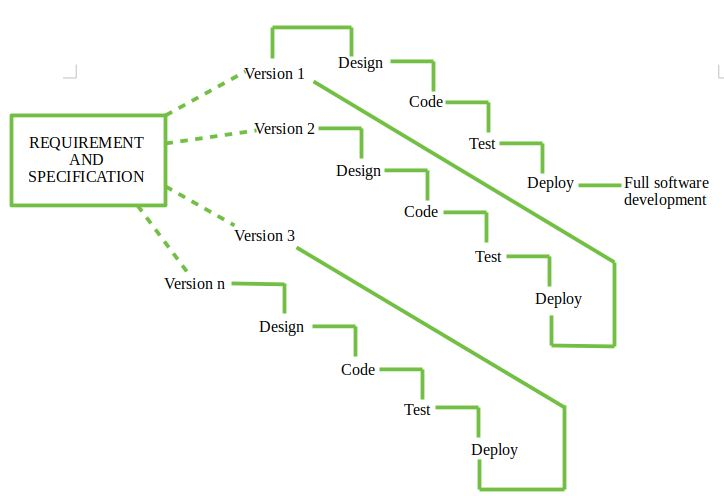
\includegraphics[width = 5in]{Proposal/static/incremental.png}
    \caption{Incremental Model}
    \label{fig:enter-label}
\end{figure}
\newpage

\begin{itemize}
    \item \textbf{Requirement Gathering:}\\
    Requirements for the System Administration Portal (SAP) project are gathered through a combination of user interviews, surveys, and consultations with students, instructors, and administrative staff.Regular feedback loops are established, enabling continuous adjustments based on evolving user expectations and emerging trends in educational technology.
    \item \textbf{Design:}\\
    The design phase of the Student Access Portal (SAP) project involves creating a detailed architectural blueprint and user interface (UI) design that aligns with the project's goals and user requirements. The structure of database is planned, use cases evaluated, user interface designed and security was integrated into the design.
    \item \textbf{Coding and Testing:}\\
    In the coding phase, we have decided to use the MERN stack.This phase involves writing clean, efficient code, integrating frontend and backend components, and implementing features. Concurrently, rigorous testing is conducted, including unit, integration, and user acceptance testing, ensuring the SAP's functionality, security, and performance align with requirements.
    \item \textbf{Deployment:}\\
    We will set up the deployment infrastructure the web application considering the cost effectiveness and efficiency. This involves setting up servers, and ensuring the platform's security measures. Once deployed, the SAP becomes accessible to users, and ongoing monitoring and maintenance processes begin to ensure optimal performance and user satisfaction.
\end{itemize}
\newpage
\subsection{System Development Tools}
\begin{itemize}
    \item \textbf{MongoDB:}\\
    MongoDB is utilized in the construction of the System Administration Portal (SAP) as the primary database management system. MongoDB, a NoSQL database, offers a flexible and scalable solution, aligning well with the dynamic requirements of the SAP. It allows us to store various types of data, including user profiles, resource metadata, room collaborations, and notifications, in a schema-less format, accommodating changes and additions without complex migrations.MongoDB's document-oriented model enables us to structure data in a way that mirrors real-world entities, such as students, instructors, courses, and resources. This enhances the efficiency of querying and retrieving data, making it well-suited for managing user profiles, room information, and resource associations. Additionally, MongoDB's support for indexing and aggregation pipelines ensures that data access remains performant as the platform scales.\cite{mongo}
    \item \textbf{ReactJS:}\\
    We preferred ReactJS as the frontend library to create dynamic, interactive user interfaces. It is preferrable due to it's benefits like: Component-based development, Efficient UI updates, Responsive Design, Ecosystem and Community, Third Party Integrations etc.\cite{node}
    \item \textbf{ExpressJS:}\\
     ExpressJS serves as the backbone of the SAP's backend, facilitating request handling, route management, middleware integration, and database interactions. Its versatility and efficiency make it an ideal choice for building a secure, responsive, and scalable backend system that complements the frontend, ensuring a cohesive and seamless user experience within the application. ExpressJS serves as the web server for the SAP, handling incoming HTTP requests, routing them to the appropriate endpoints, and responding with the required data.Express simplifies route handling, allowing us to define clear and structured routes for various API endpoints.Express middleware enables us to process requests before they reach the intended route, facilitating tasks such as authentication, data validation, error handling, and logging. This ensures a secure and efficient backend operation.Express simplifies the creation of robust APIs, making it efficient to expose functionalities to the frontend (built with ReactJS) and other components of the application.\cite{express}
    \item \textbf{NodeJS:}\\
    Node.js serves as the backbone that powers the SAP's responsiveness, scalability, and real-time capabilities. Its single language approach, non-blocking architecture, and extensive ecosystem make it an ideal choice for creating a modern, efficient, and highly interactive educational platform that serves both students and instructors effectively. Node.js enables the use of JavaScript on both the client and server sides, ensuring consistency and reducing the need for context-switching between languages.  Node.js employs a non-blocking, event-driven architecture, making it highly efficient in handling asynchronous tasks.Node.js is known for its ability to handle a large number of concurrent connections with minimal resource usage.Node.js is well-suited for building microservices and RESTful APIs, aligning with the architecture of the SAP. Node.js's event-driven nature makes it an excellent choice for real-time applications.\cite{node}
    \item \textbf{GitLab:}\\
    GitLab is selected for the development of the SAP due to its robust version control, code collaboration features, CI/CD capabilities, project management tools, and options for self-hosting. These aspects make GitLab a comprehensive platform that enhances the efficiency, security, and collaboration of the development process, aligning well with the goals of the SAP project.As for choosing GitLab over GitHub, there are several factors to consider. GitLab offers a more comprehensive feature set in its free plan, including built-in CI/CD pipelines and project management tools. This is advantageous for a project like the SAP, where an integrated development environment is crucial. Additionally, GitLab's self-hosting option provides us with greater control over our repositories, which can be essential for data privacy compliance.\cite{gitlab}
\end{itemize}
\newpage

\begin{center}
\section{SYSTEM DESIGN AND ARCHITECTURE}
\end{center}
\subsection{Use Case Diagram:}
\begin{figure}[h]
    \centering
    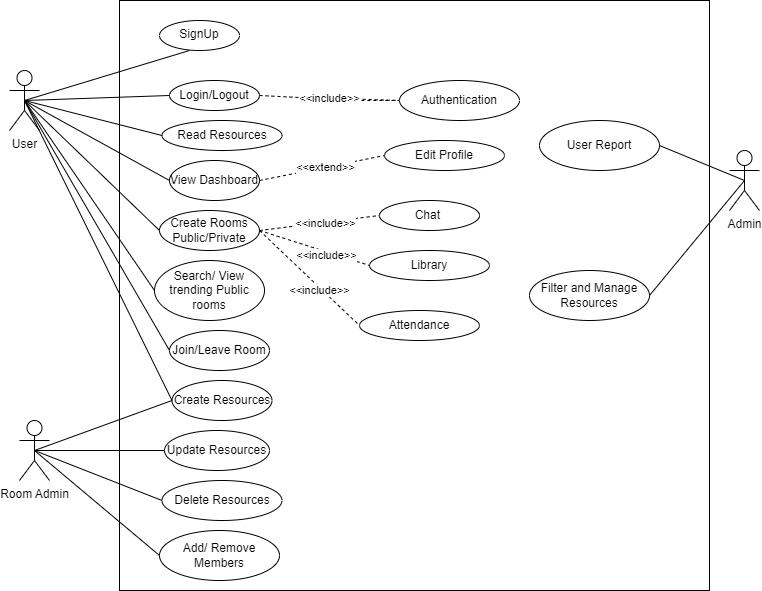
\includegraphics[width=6in, height=6in]{Proposal/static/use_case_sap.drawio.png}
    \caption{Use Case Diagram for SAP}
    \label{fig:enter-label}
\end{figure}
\newpage

\subsection{Data Flow Diagrams:}
\begin{figure}[h]
    \centering
    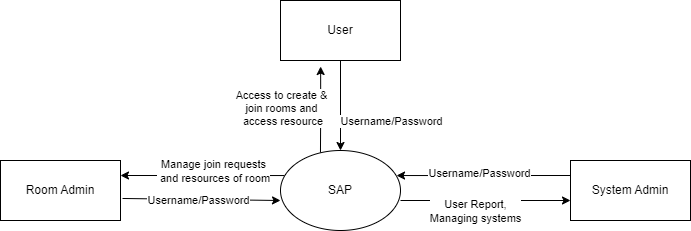
\includegraphics[width=6in, height=4in]{Proposal/static/dfd_0.png}
    \caption{Level 0 DFD}
    \label{fig:enter-label}
\end{figure}
\newpage

\begin{figure}[h]
    \centering
    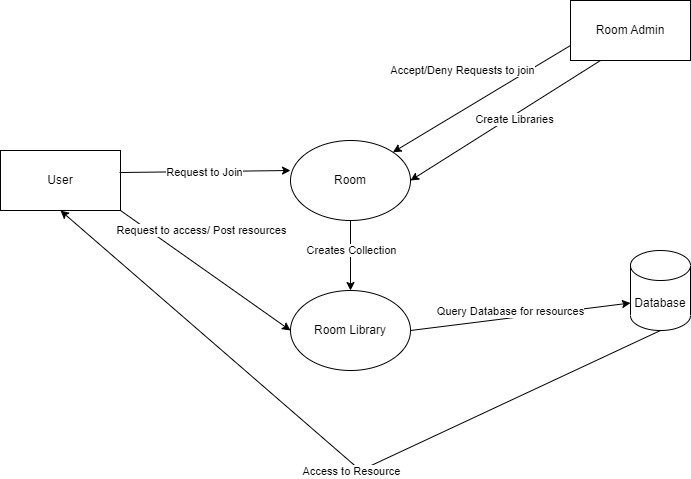
\includegraphics[width=6in, height=4in]{Proposal/static/dfd_1.png}
    \caption{Level 1 DFD}
    \label{fig:enter-label}
\end{figure}
\newpage

\subsection{Sequence Diagram:}
\begin{figure}[h]
    \centering
    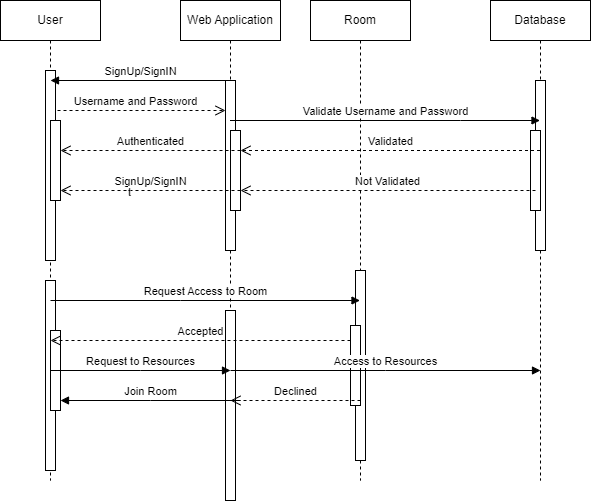
\includegraphics[width=6in, height=6in]{Proposal/static/Sequence_diagram_SAP.drawio.png}
    \caption{Sequence Diagram}
    \label{fig:enter-label}
\end{figure}
\newpage

\subsection{Activity Diagram:}
\begin{figure}[h]
    \centering
    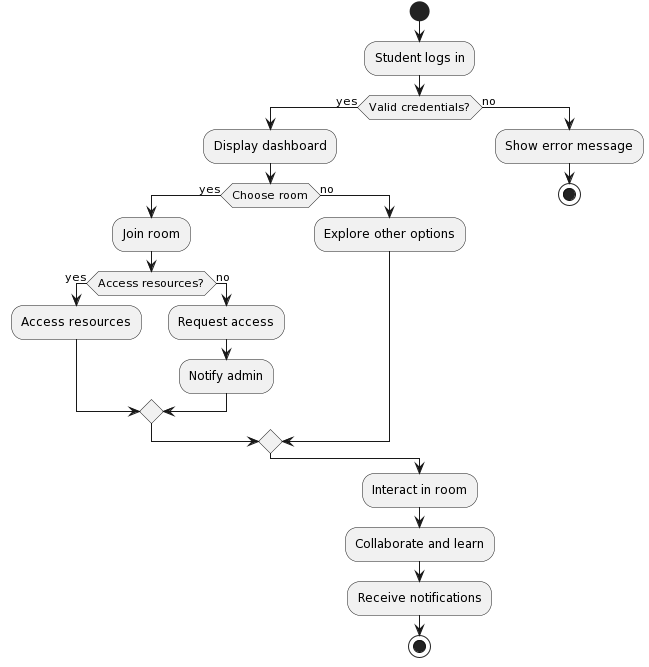
\includegraphics[width=6in, height=6in]{Proposal/static/activity_diagram_sap.png}
    \caption{Activity Diagram}
    \label{fig:enter-label}
\end{figure}
\newpage

\subsection{Class Diagram:}
\begin{figure}[h]
    \centering
    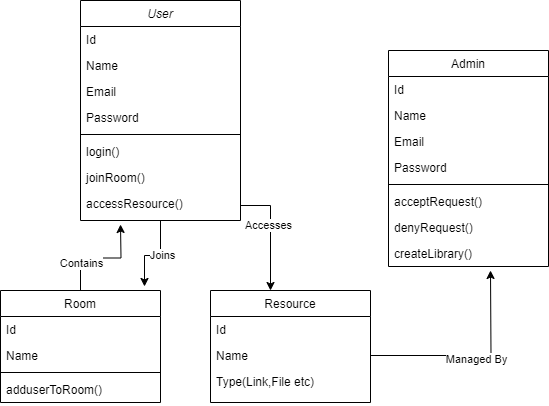
\includegraphics[width=6in, height=6in]{Proposal/static/Class_Diagram.png}
    \caption{Class Diagram}
    \label{fig:enter-label}
\end{figure}
\newpage

\subsection{ER Diagram:}
\begin{figure}[h]
    \centering
    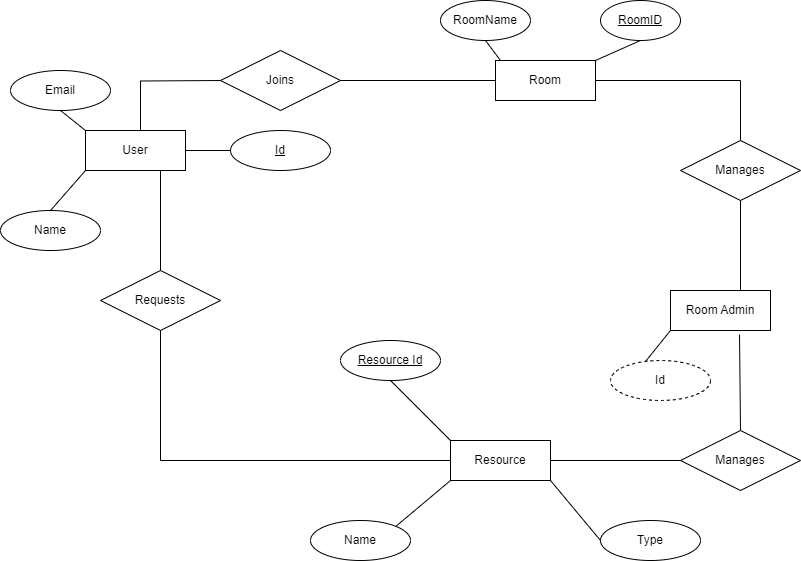
\includegraphics[width=6in, height=6in]{Proposal/static/ER.png}
    \caption{ER Diagram}
    \label{fig:enter-label}
\end{figure}
\newpage

\begin{center}
\section{EXPECTED RESULT}
\end{center}
The Student Access Portal (SAP) is poised to deliver transformative results to the educational experience. By providing a centralized platform for students to access resources, collaborate within virtual rooms, and receive timely updates, the SAP will significantly enhance student engagement, academic performance, and overall satisfaction. Students will experience streamlined resource management, simplified navigation, and personalized dashboards that empower them to tailor their learning journey. The SAP's seamless integration with both classroom and remote learning ensures continuity in education, especially in challenging times. Instructors will benefit from real-time resource updates, engagement monitoring, and data-driven insights, enabling them to refine teaching strategies and better support students. The SAP's promotion of technology literacy, its responsive design, and ongoing innovation will equip students with essential skills for the digital age, enhancing their readiness for the workforce. Ultimately, the SAP's comprehensive approach fosters a dynamic, interactive, and efficient educational ecosystem, creating a positive impact on both students and instructors, and shaping the future of education.The SAP's versatility in supporting both classroom and remote learning is a critical aspect that ensures educational continuity, a lesson learned from recent disruptions. This adaptability, combined with the SAP's focus on resource management, will enable students to seamlessly transition between learning modes, ensuring uninterrupted access to vital course materials and promoting a consistent educational experience.
Instructors will benefit from the real-time updates and engagement monitoring features within the SAP. This will provide valuable insights into student interactions, enabling instructors to tailor their teaching strategies, identify areas where additional support is needed, and ultimately elevate the quality of education provided. The SAP's data-driven approach empowers instructors to make informed decisions, leading to improved teaching effectiveness and student outcomes.
\newpage

\begin{center}
\section{LIMITATIONS}
\end{center}
\begin{itemize}
    \item The effectiveness of the SAP relies on students having access to digital devices and a stable internet connection. In areas with limited technological infrastructure, some students may face challenges in fully utilizing the platform, potentially leading to unequal access to educational resources.
    \item While efforts will be made to create an intuitive user interface, some users, particularly those less familiar with technology, might experience a learning curve when navigating the SAP. Adequate training and support mechanisms will be essential to address this potential challenge.
    \item Encouraging widespread adoption among students, instructors, and administrative staff is essential for the SAP's success. Overcoming potential resistance to change, ensuring proper training, and effectively communicating the benefits of the platform are challenges that must be addressed.
\end{itemize}
\newpage
\newpage

\printbibliography[heading=mybibliography]
\end{document}
